\documentclass[11pt,oneside,final,notitlepage,a4paper,wide]{mwart}
\usepackage[utf8]{inputenc}	% Pakiet pozwalający kodować znaki diakrytyczne w różnych wariantach - https://ctan.org/pkg/inputenc
\usepackage{polski} 		% Pakiet dodający język polski - https://ctan.org/pkg/polski
\usepackage{graphicx}		% Pakiet oferujący dodatkowe funkcje przy dodawaniu grafik - https://ctan.org/pkg/graphicx
\usepackage{setspace}		% Pakiet zapewniający dodatkowe ustawienia odstępów w dokumencie - https://ctan.org/pkg/setspace

\usepackage[]{hyperref}		% Pakiet umożliwiający dodatkowe ustawienia pliku pdf - https://ctan.org/pkg/hyperref
\usepackage{xcolor}		% Pakiet dodający dodatkowe ustawienia kolorów - https://ctan.org/pkg/xcolor
\usepackage{makeidx}		% Pakiet umożliwiający tworzenie indeksów - https://ctan.org/pkg/makeidx

	%------------------------------------------------------------------------------%
					% Do uzupełnienia %
	%------------------------------------------------------------------------------%

\onehalfspacing			% Ustawienie pojedynczego odstępu między linijkami.
\setlength{\parindent}{1.25cm}	% Rozmiar wcięcia akapitów.
\renewcommand{\labelitemi}{$\bullet$} % Ustawienie kropki jako punktatora listy {itemize}.

\title{Wyznaczanie ogniskowej soczewki skupiającej} 
\author{JanekR\underline{\hspace{0.2cm}}Prorok}
\date{\today}

\definecolor{orangelink}{rgb}{0.7,0.18,0.1} % Zdefiniowany własny kolor - tu wykorzystany do linków.
	
\hypersetup{			% Ustawienia pliku pdf - http://www.tug.org/applications/hyperref/manual.html#x1-120003.8
    pdftitle={Wyznaczanie ogniskowej soczewki skupiającej}, % title
    pdfdisplaydoctitle=true,	% display document title instead of file name in title bar
    pdfauthor={JanekR_Prorok},	% author
    pdfsubject={},		% subject of the document
    pdfcreator={Texmaker, MiKTeX}, % creator of the document
    pdfproducer={},		% producer of the document
    pdfinfo={},			% Alternative interface for setting the document information
    pdfkeywords={},		% list of keywords    
    bookmarks=true,		% show bookmarks bar?
    bookmarksnumbered=true,     % put section numbers in bookmarks
    bookmarksopen=true,       	% open up bookmark tree
    bookmarksopenlevel=1,	% level to which bookmarks are open
    pdfpagelabels=true,		% set PDF page labels                   
    pdfpagemode=UseOutlines,	% Determines how the file is opening in Acrobat; the possibilities are UseNone, UseThumbs (show thumbnails), UseOutlines (show bookmarks), FullScreen, UseOC (PDF 1.5), and UseAttachments (PDF 1.6). If no mode if explicitly chosen, but the bookmarks option is set, UseOutlines is used.
    unicode=true,		% non-Latin characters in Acrobat’s bookmarks
    pdftoolbar=true,		% show Acrobat’s toolbar?
    pdfmenubar=true,		% show Acrobat’s menu?
    pdffitwindow=false,		% window fit to page when opened
    pdfstartview=Fit,		% fits the width of the page to the window
    pdfnewwindow=true,		% links in new PDF window
    colorlinks=true,		% false: boxed links; true: colored links
    linkcolor=orangelink,	% color of internal links (change box color with linkbordercolor)
    citecolor=orangelink,	% color of links to bibliography
    filecolor=orangelink,	% color of file links
    urlcolor=orangelink,	% color of external links
    pdfpagelayout=OneColumn,	% set layout of PDF pages
    % pdfstartpage=1,		% page at which PDF document opens
    % pdfnumcopies=,		% number of printed copies
    % filebordercolor=,		% color of border around file links
    % filecolor=,		% color of file links
    % linkbordercolor=,		% color of border around links
    % menubordercolor=,		% color of border around menu links
    % menucolor=,		% color for menu links
    % pagebackref=,		% backreference by page number
    % pdfcenterwindow=false,	% position the document window in the center of the screen
    % pdfdirection=,		% direction setting   
    % baseurl=,			% Sets the base URL of the PDF document
    % pdftrapped=,		% Sets the document information Trapped entry. Possible values are True, False and Unknown. An empty value means, the entry is not set.
}

% The pdfpagelayout can be one of the following values.
	% SinglePage - Displays a single page; advancing flips the page
	% OneColumn - Displays the document in one column; continuous scrolling.
	% TwoColumnLeft - Displays the document in two columns, odd-numbered pages to the left.
	% TwoColumnRight - Displays the document in two columns, odd-numbered pages to the right.
	% TwoPageLeft	- Displays two pages, odd-numbered pages to the left (since PDF 1.5).
	% TwoPageRight - Displays two pages, odd-numbered pages to the right (since PDF 1.5).
% Dokumentacja: http://www.tug.org/applications/hyperref/manual.html

	%%%%%%%%%%%%%%%%%%%%%%%%%%%%%%%%%%%%%%%%%%%%%%%%%%%%%%%%%%%%%%%%%%%%%
	
\begin{document}
% \sloppy - Wymuszenie nieprofesjonalnego trzymania się w marginesach (kosztem dziwnie rozciągniętych odstępów).

	\begin{center}
	 	\LARGE{\textbf{Wyznaczanie ogniskowej soczewki skupiającej}}\\ \medskip
 		\small{JanekR\underline{\hspace{0.2cm}}Prorok}
	\end{center}
\section{Wstęp}
	Celem doświadczenia jest wyznaczenie ogniskowej soczewki skupiającej na podstawie pomiaru odległości przedmiotu i otrzymanego obrazu od soczewki.
%
	\subsection{Podstawy teoretyczne}
		Soczewka jest to proste urządzenie optyczne, zwykle szklane. Soczewki szklane, jeśli ich grubość jest większa przy ich osi niż przy brzegach, są soczewkami skupiającymi. Gdy soczewka skupia równoległą wiązkę światła, po przejściu przez nią, promienie spotykają się w jednym punkcie, nazywanym \emph{ogniskiem} i oznaczanym $F$. Odległość ogniska od środka soczewki nazywamy \emph{ogniskową}.
		\begin{figure}[h]
			\centering
			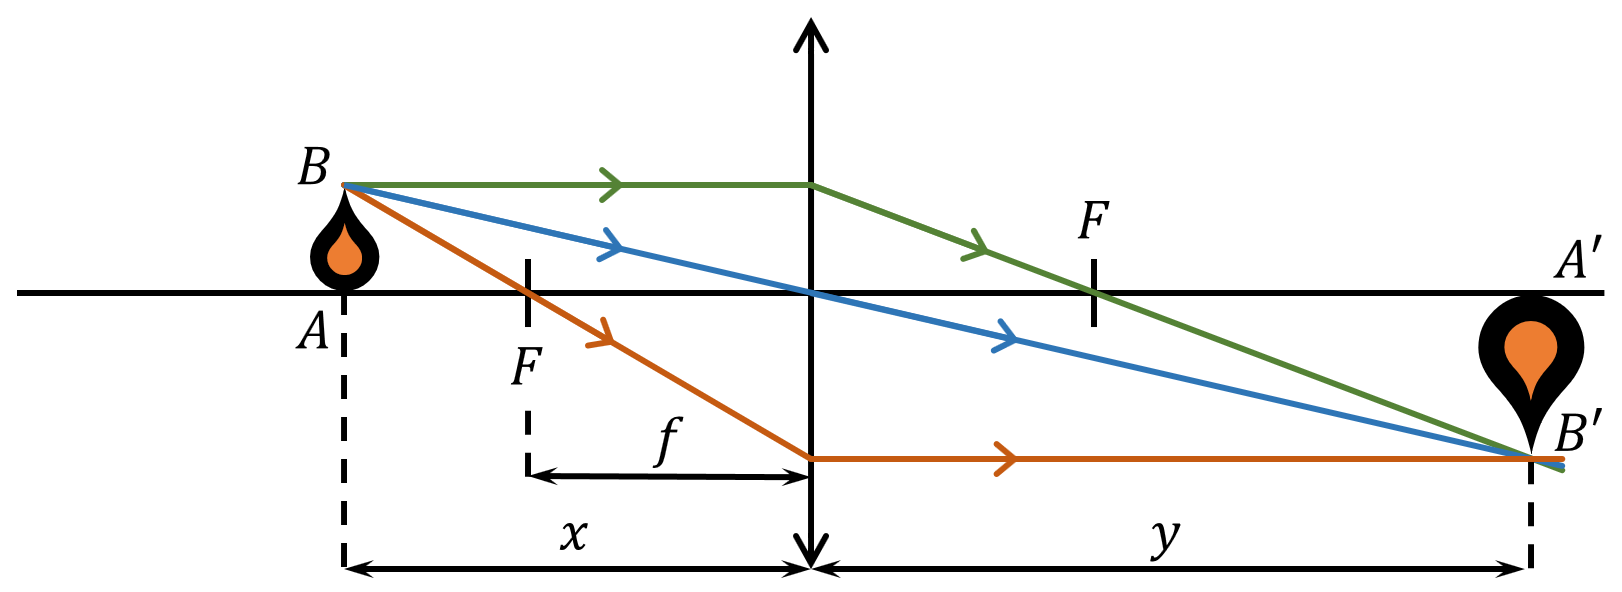
\includegraphics[width=\textwidth]{rys/schemat_powstawania_obrazu.png}
			\caption{Schemat powstawania obrazu w soczewce skupiającej}
		\end{figure}
	
		Zależność pomiędzy odległością przedmiotu od soczewki, a odległością jego obrazu otrzymanego w tej soczewce opisuje \emph{równanie soczewki}:
		\begin{equation}
			\frac{1}{f} = \frac{1}{x} + \frac{1}{y}
		\end{equation}
		gdzie:
		\begin{itemize}		
			\item[$f$] ogniskowa soczewki,
			\item[$x$] odległość przedmiotu od soczewki,
			\item[$y$] odległość obrazu od soczewki.
		\end{itemize} \smallskip
	
		Mierząc odległość przedmiotu od soczewki i odległość obrazu od soczewki można wyznaczyć ogniskową przekształcając powyższy wzór:
		\begin{equation}
			f = \frac{xy}{x + y} \label{wzór.f}
		\end{equation}
%
\section{Metoda obserwacji zjawiska}
	\subsection{Elementy zestawu doświadczalnego}
		\begin{itemize}
			\item zapalona świeczka,
			\item soczewka skupiająca, o ogniskowej deklarowanej przez producenta $f = +13,6 \ cm$,
			\item ekran -- biała kartka,
			\item centymetr krawiecki.
		\end{itemize}
		\begin{figure}[h]
			\centering
			\includegraphics[width=\textwidth]{rys/schemat_zestawdoswiadczalny}
			\caption{Schemat zestawu doświadczalnego}
		\end{figure}
	\subsection{Przebieg doświadczenia}
		Na płaskiej powierzchni umieszczono, w jednej linii, zapaloną świeczkę oraz soczewkę w pewnej odległości. Następnie dopasowano odległość ekranu od soczewki, aż do uzyskania ostrego obrazu świeczki i zmierzono odległości. Wyniki pomiaru zapisano w tabeli. Powyższe pomiary przeprowadzono dla pięciu różnych odległości. 
%
\section{Wyniki pomiarów}
	Odległość mierzono papierowym centymetrem krawieckim o dokładności pomiaru $\Delta x = 0,5 \ cm$, $\Delta y = 0,5 \ cm$.
	\begin{table}[h]
		\centering
		\begin{tabular}{c|c|c}
			Lp. & $x \left[ cm \right]$ & $y \left[ cm \right]$ \\ \hline
			1 & $20,5$ & $31,0$ \\
			2 & $29,0$ & $22,5$ \\
			3 & $24,5$ & $26,5$ \\
			4 & $17,0$ & $41,0$ \\
			5 & $37,0$ & $20,5$ \\
		\end{tabular}
		\caption{Wyniki pomiarów}
	\end{table}
%
\section{Opracowanie wyników pomiarów}
	\subsection{Obliczenia}
		Wartość ogniskowej obliczono korzystając ze wzoru (\ref{wzór.f}).
		
		Przykładowe obliczenie wartości ogniskowej
		\begin{equation}
			f = \frac{20,5 \ cm \cdot 31,0 \ cm}{20,5 \ cm + 31,0 \ cm} = \frac{635,5 \ cm^{2}}{51,5 \ cm} \approx 12,34 \ cm 
		\end{equation}
		
		Pozostałe wartości obliczonych ogniskowych przedstawiono w tabeli poniżej.
		\begin{table}[h]
			\centering
			\begin{tabular}{c|c}
				Lp. & $f \left[ cm \right]$ \\ \hline
				1 & $12,34$ \\
				2 & $12,67$ \\
				3 & $12,73$ \\
				4 & $12,02$ \\
				5 & $13,19$ \\
			\end{tabular}
			\caption{Wyniki obliczeń wartości ogniskowej}
		\end{table}
		
		Średnia arytmetyczna powyższych wyników $Sr_{f_{1-5}} = 12,59 \ cm$
%
	\subsection{Analiza niepewności pomiarowej}
		\subsubsection{Źródła niepewności}
			Na wynik pomiarów mogły mieć wpływ następujące składowe:
			\begin{itemize}
				\item niedoskonałość metody pomiarowej,
				\item błędy w odczycie wskazań przyrządów,
				\item dokładność przyrządów pomiarowych,
				\item zastosowane przybliżenia.
			\end{itemize}
		\subsubsection{Rachunek niepewności pomiarowej}
			Do obliczenia niepewności pomiarowej wykorzystano wzór na niepewność maksymalną
			\begin{equation}
				\Delta f = \frac{f_{max} - f_{min}}{2} = \frac{13,19 \ cm - 12,02 \ cm}{2} = 0,585 \ cm
			\end{equation}
%
	\subsection{Wynik końcowy}	
		Wartość ogniskowej soczewki skupiającej obliczona w doświadczeniu
		\begin{equation}
			f = \left( 12,59 \pm 0,585 \right) cm
		\end{equation}
%
\section{Wnioski i podsumowanie}
	Wykorzystana metoda pozwoliła wyznaczyć ogniskową soczewki skupiającej. Wyniki są zbliżone do wartości deklarowanej przez producenta soczewki. Metoda ta jest w miarę dokładna -- niepewność względna jest rzędu $ 3,125 - 11,728 \% $.
	
	Największy wpływ na dokładność wyników miała przede wszystkim niedoskonałość metody pomiarowej. Ekran nie zawsze był ustawiony idealnie prostopadle do płaszczyzny podstawy zestawu doświadczalnego. Dla dokładniejszych pomiarów należałoby zastosować ławę optyczną.
%
\section{Źródła}
	\begin{itemize}
		\item Nowa Era, \emph{Zrozumieć fizykę 3}, Warszawa 2017, s. 289, 298
		\item Centralna Komisja Egzaminacyjna, \emph{Wybrane wzory i stałe fizykochemiczne na egzamin maturalny z biologii, chemii i fizyki}, Warszawa 2015, s. 7
	\end{itemize}
\end{document}
